  
\subsubsection{Parallel Rheobase Solver}

The Rheobase determination algorithm was in fact a specific instance of a more general type of algorithm, one that finds the current injection that causes a pre-determined number of spikes.

\begin{figure}    
  \begin{center}
  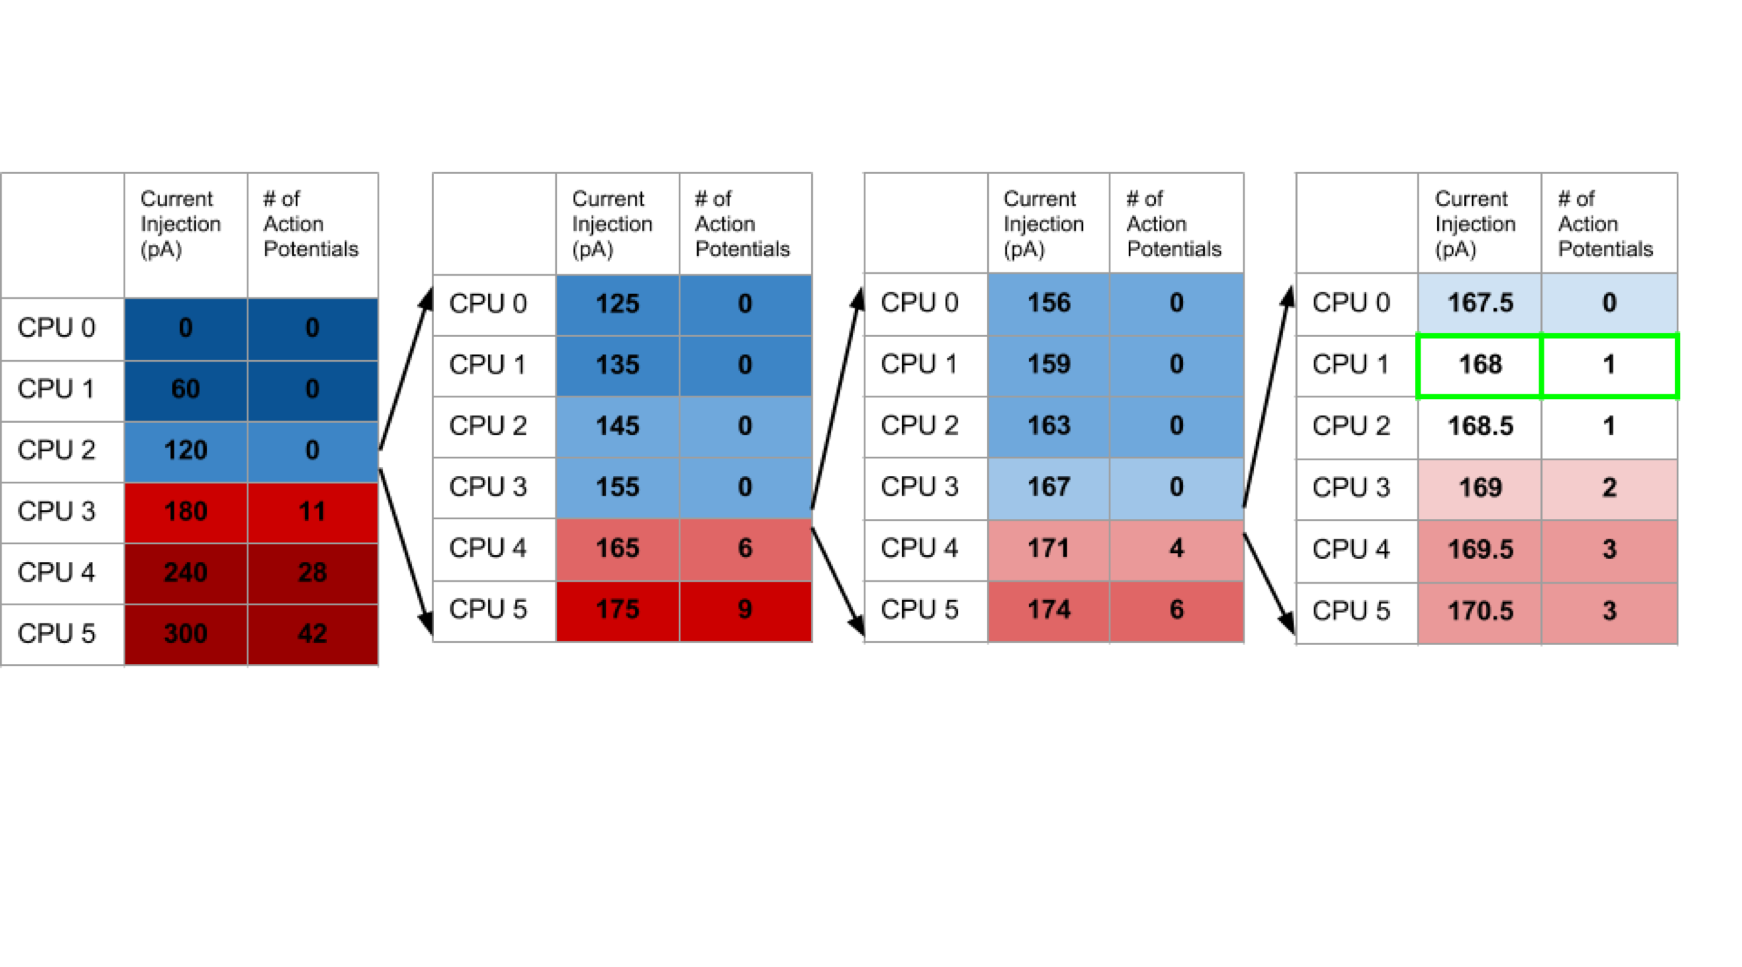
\includegraphics[width=0.7\linewidth]{{figures/rheobase_algorithm.png}}
    \caption{We developed a generic algorithm which took models, and found the minimal current injection value that would cause only one spike. The normal structure of this algorithm is a binary search, however we modified the algorithm so it would map onto multiple processors at once. This lead to significant speed ups for multicompartment NEURON models}

  \end{center}
\end{figure} 
    
Below I show that for multi-compartment neuron models using a parallel Rheobase algorithm adds a significant speed up to rheobase solution evaluation. It
is important to consider that determinig rheobase usually involves
between 10-35 model simulations at different current injection
strengths. Whereas the remaining error score calculations only involve
at most one model evaluation each. Consider an optimization problem where
there are only eight error scores to calculate, and four of the eight
errors are for non spiking simulations of less than 500ms, a rheobase
simulation is for 1200ms, and it involves both non-spiking and
multi-spiking behavior. Multi-spiking models take longer to simulate
than non spiking and single spiking models for the simple reason that $\frac{dV_{M}}{dt}$ changes rapidly and solvers that are capable of variable time steps, will not be able to exploit sparse sampling in these rapid changes of  $\frac{dV_{M}}{dt}$. In this particular
instance where finding the unique rheobase value for each different gene
is important, that rheobase determination is the biggest computational
bottleneck to  optimization, because it implies approximately 20-30 model evaluations.

It is also important to consider that the speed of model simulation is
often determined by the exact parameterization of the model in question.
During optimization parameterization frequently changes. Multi-spiking
models that are slower to evaluate are frequently sampled by a genetic
algorithm optimizer.

parallel Rheobase search time NEURON  $4.8$
serial Rheobase search time NEURON  $18.7$
Approximate speed up $\times 3.9$

Brian2 adaptive Exponential model   
elapsed serial:  $0.7914438247680664$
elapsed parallel: $ 0.2590057849884033$
speed up parallel:   $\times 3.0$

Algorithm was able to speed up this slow NEURON unit code. $ \frac{73}{19} $ represents a substantial speed up. of about 3.8. This is consistent with previous work.

This approach solving Rheobase was later generalized to an algorithm find current injection values that would cause any arbitrary number of spikes, as this was necessary for speeding up supra threshold optimizations \url{https://github.com/russelljjarvis/neuronunit/blob/master/neuronunit/tests/target_spike_current.py}.
%$ array(51.79317142) * pA$

 